%The use case scenario is based on a previously published paper in the \emph{Journal of Applied Intelligence} \cite{baouyageneration2022} for smart water flow assessment. The industrial case study involves the Cecebre dam infrastructure located in Spain. The primary objective of this dam is to collect water from the Meirama Lake and store it in the Cecebre Reservoir from the city of La Coruña; this reservoir plays a vital role in meeting water supply demands for various purposes. Three sensor nodes gather and transmit diverse measurements such as water level (WL), water volume (WV), and rain precipitation (RP) payload to the Fog system to assess the water flow (WF). The internal digital architecture of the industrial use case is partially depicted in \fig{rabbitarchitecture}. The deployment of RabbitMQ on the Sensinact gateway has not yet been completed. As a result, questions regarding the feasibility of this deployment are being addressed and explored in our study. We aim to gain a deeper understanding of potential attack impact. 

In the context of our experiments, we refer to a use case scenario from the collaborative European research project~\cite{brainiot2022} for smart water flow assessment. Three sensor nodes gather and transmit diverse measurements such as water level (WL), water volume (WV), and rain precipitation (RP) payload to the Fog system through 
the Sensinact gateway~\cite{sensinactref2024} to assess the water flow (WF). The internal digital architecture of the industrial use case is partially depicted in \fig{fig:rabbitarchitecture}. 
The deployment of RabbitMQ on the Sensinact gateway has not yet been completed. As a result, questions regarding the feasibility of this deployment are being addressed and explored in our study. 
We aim to gain a deeper understanding of the potential impact of an attack.  

% In the context of our experiment, we used the algorithm (ref) to compute the attacks freqnecices and used them as a parameter for CSG models.... 

The requirements described below are a summary (with some revisited information) of the security properties of RabbitMQ. They are expressed as a set of properties in natural language to protect the corresponding assets.
\begin{boxF}
\begin{itemize}
    \item \emph{\bfseries{Property 1}}: When the sensors transmit payload messages ($wv$, $wl$, and $rp$ $\in [1\ldots3]$) to the fog, we are interested in determining the probability of payload tampering at each round.
    \item \emph{\bfseries{Property 2}}: When the sensors transmit payload ($wv$, $wl$, and $rp$ $\in [1\ldots3]$) messages to the fog, our objective is to determine the probability of message loss after each round.
    \item \emph{\bfseries{Property 3}}: When the sensors transmit payload ($wv$, $wl$, and $rp$ $\in [1\ldots3]$) messages to the fog, Our objective is to determine the probability of message loss caused by the unrouted payload after each round (Tampering affecting only routing keys).
\end{itemize}
\end{boxF}
We intend to provide a formal specification of the functional and security requirements for message delivery that RabbitMQ must fulfill to ensure its effectiveness. We will consider DoS, MITM ARP spoofing, and Mirai attacks at southbound bridges (sensors) and queues. 


\subsection{\cmt{Experimental setup}}
\cmt{Our analyses rely on PRISM-games v4.7, where experiments are conducted on an Ubuntu-I7 system with 32GB RAM. The system model is accessible via the link provided in \cite{edcc23} and adheres to the \emph{CSG} formalism supported by PRISM-games. The engine is set to \quot{Explicit}; other engines are supported by PRISM that offers performance regarding model structure (Please refer to documentation). Player definitions within the model are identified by \quot{player tag} delimiters. For example, the player \texttt{p1} represents the attacker, as exemplified in: \texttt{player p1  Attacker endplayer}. Parameters associated with data manipulation attacks are derived from the dataset denoted as \quot{\texttt{C1}} in \cite{edcc23}. The selection of attack frequency hinges on the chosen scenario, declared as a \texttt{const int} variable. For instance, scenario 1 corresponds to DDoS attacks, scenario 2 to ARP attacks, and scenario 3 to Mirai attacks. A dedicated Python code was developed to calculate the attack rate based on this dataset. Properties relative to our models are expressed in the Modeling section.}


% \cmt{For our analyses, we utilized PRISM-games v4.7, where all experiments were performed on an Ubuntu-I7 system equipped with 32GB of RAM. The system model used in our study can be accessed via the provided link \cite{edcc23}. The PRISM model is \texttt{CSG} supported by PRISM-games. The Engine deleted is \quot{Explicit}. The players definitions in the model are expressed between player tag definition. for instance the player \texttt{p1} refers to the attacker in : \texttt{player p1  Attacker endplayer}. Parameters associated with attacks involving data modification were obtained from the dataset referenced as \quot{\texttt{C1}} in \cite{edcc23}. The selection of the attack frequency is based on the selected scenario (declared as \texttt{const int} ), for instance secanri takes 1 for DDoS 2 for ARP and 3 for Mirai attacks. A Python code was developed to calculate the attack rate based on this dataset}.

\subsection{Modeling}
\label{prop:validation}
%We intend to provide an informal overview of the functional and security requirements for message delivery that RabbitMQ must fulfill to ensure its effectiveness. In our analyses, we utilized PRISM-games v4.7. All experiments were conducted on an Ubuntu-I7 system with 32GB of RAM. The modeled system is available at the link: \cite{edcc23} with reference \texttt{M3}. Parameters related to attacks involving data modification were collected from the dataset provided in \cite{edcc23} under reference \texttt{C1}. A Python code was developed to compute the attack rate using this dataset. 

The RabbitMQ models are partitioned into two distinct models to analyze the impacts of threats on different components of the architecture, specifically the southbound bridges (\quot{M3}) and queues (\quot{M4}). This division is essential to address the challenges of the state space explosion.



We enhance the model by incorporating an integer constant as in \cite{KNPS19} and a module (see \lst{lst:rounds}) to keep track of the number of rounds. In this case, as the commands are unaffected by the players' choices, they are considered unlabelled with empty action. Consequently, these commands are executed regardless of the actions taken by the players. Furthermore, the module is deterministic due to the disjoint guards present in both commands.
\lstset{
    breaklines=true,
    style=framed,
    escapeinside={<@}{@>},
    morekeywords={void, int, public, private, class, protected, submodules, network, connections, const, init, int, bool, double, module, rewards, endrewards, endmodule},
    basicstyle=\ttfamily,
    keywordstyle=\bfseries\color{blue},
        morecomment=[f][\color{green!30!black}][0]{/*},
    morecomment=[l][\color{green!30!black}]{//},
    label=queueemodel
}

\begin{figure}[!htb]            
\begin{minipage}{16.5cm}
\begin{lstlisting}[style=framed,%customc, 
caption=Rounds module to Express multiple Tentatives ,
 	label=lst:rounds]	
const k; // number of rounds
module rounds // module to count the rounds
 rounds : [0..k+1];
 [] rounds<=k -> (rounds'=rounds+1);
 [] rounds=k+1 -> true;
endmodule
\end{lstlisting}
 \end{minipage}  
\end{figure}




\cmt{The properties are defined as a set of requirements in rPATL, mapped from the original natural language expressions in the use case}.

%\emph{\bfseries{REQ1}}: When the sensors transmit payload messages ($wv$, $wl$, and $rp$ $\in [1\ldots3]$) to the fog, we are interested in determining the probability of payload tampering at each round.

 
	    
	    \begin{resp}{\textbf{\textit{Property 1}}}
        \begin{equation}
        \label{eq1}
        \mathtt{\gl{\gl{\textcolor{red}{p1},\textcolor{red}{p2}}}Pmax=? [ !\quot{\textcolor{red}{payload\_tamper}} U \quot{\textcolor{red}{payload\_tamper}}  ]}, \mathtt{\ \textcolor{red}{rounds}=\textcolor{blue}{1}:\textcolor{blue}{30}:\textcolor{blue}{1}} 
        \end{equation}
        \end{resp}
       
        
% \emph{\bfseries{REQ2}}: When the sensors transmit payload ($wv$, $wl$, and $rp$ $\in [1\ldots3]$) messages to the fog, our objective is to determine the probability of message loss after each round.
 
	   
	    \begin{resp}{\textbf{\textit{Property 2}}}
        \begin{equation}
        \label{eq2}
        \splitdfrac{\mathtt{ \gl{\gl{\textcolor{red}{p1}}}R{\{\quot{\textcolor{red}{damage}}\}}max=? [ F \ \textcolor{red}{r}=\textcolor{red}{rounds} ]/}}{\mathtt{\ \gl{\gl{\textcolor{red}{p2}}}R{ \{\quot{\textcolor{red}{sent}}\}}max=? [ F\ \textcolor{red}{r}=\textcolor{red}{rounds} ],  \ \textcolor{red}{rounds}=\textcolor{blue}{1}:\textcolor{blue}{30}:\textcolor{blue}{1}}}
        \end{equation}
        \end{resp}
        

In the context of reward structure, \quot{damage} refers to intercepted and corrupted messages, while total messages \quot{sent} by sensors represent the overall number of messages transmitted.
        
% \emph{\bfseries{REQ3}}: When the sensors transmit payload ($wv$, $wl$, and $rp$ $\in [1\ldots3]$) messages to the fog, Our objective is to determine the probability of message loss caused by the unrouted payload after each round (Tampering affecting only routing keys).
 
	   
	    \begin{resp}{\textbf{\textit{Property 3}}}
        \begin{equation}
        \label{eq3}
        \splitdfrac{\mathtt{ \gl{\gl{\textcolor{red}{p1},\ldots,\textcolor{red}{p8}}}R{\{\quot{\textcolor{red}{empty}}\}}max=? [ F \ \textcolor{red}{r}=\textcolor{red}{rounds} ]/}}{\mathtt{\ \gl{\gl{\textcolor{red}{p1},\ldots,\textcolor{red}{p8}}}R{ \{\quot{\textcolor{red}{sent}}\}}max=? [ F\ \textcolor{red}{r}=\textcolor{red}{rounds} ],  \ \textcolor{red}{rounds}=\textcolor{blue}{1}:\textcolor{blue}{30}:\textcolor{blue}{1}}}
        \end{equation}
        \end{resp}
       
        
By \quot{empty} rewards, we refer to the state of queues that are not filled with the corresponding payload.   

\subsection{Experiments and analysis of the results}

\noindent
    \begin{figure}[!htb]
    \centering
       \begin{tabularx}{\linewidth}{ m{8cm}   m{8cm}  }
           
\noindent
 \begin{minipage}[t]{8cm}
     \centering

    \includegraphics[width=180pt, height =110pt]{Graph1.pdf}
    \caption{Verification of Property \ref{eq1}.}
    \label{fig:01}
   \end{minipage}
    
           &
\noindent
   \begin{minipage}[t]{8cm}
     \centering
   		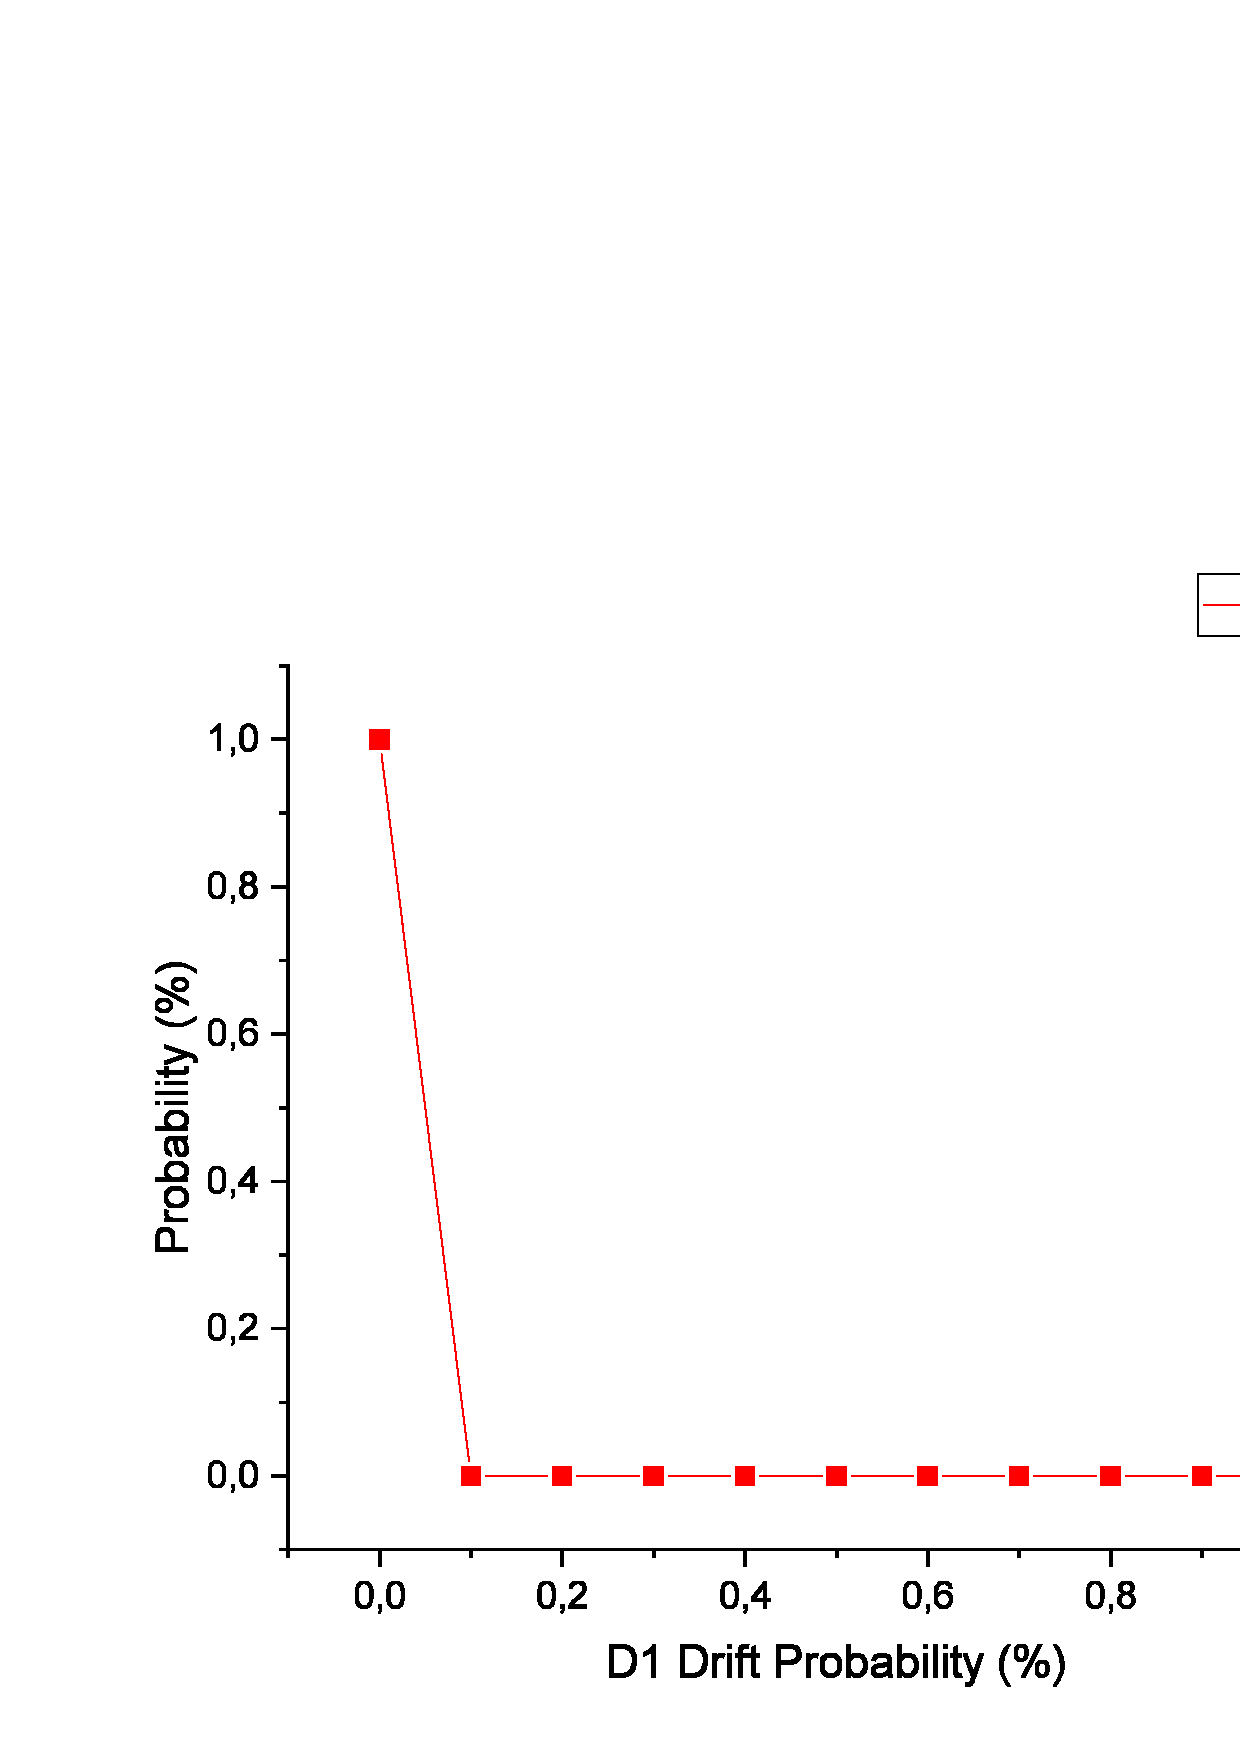
\includegraphics[width=200pt, height =110pt]{Graph2.pdf}
    \caption{Verification of Property \ref{eq2}.}
    \label{fig:02}
   \end{minipage}

       \\ 
    
           \end{tabularx}
\end{figure}

\noindent
    \begin{figure}[!htb]
       \begin{tabularx}{\linewidth}{ m{8cm}   m{8cm} }
           
%\noindent
 \begin{minipage}[t]{8cm}
     \centering

    \includegraphics[width=180pt, height =110pt]{Graph3.pdf}
    \caption{Verification of Property\ref{eq3}.}
    \label{fig:03}
   \end{minipage}
    
           &
%\noindent
   \begin{minipage}[t]{8cm}
     \centering
   		\includegraphics[width=200pt, height =110pt]{Graph4.pdf}
    \caption{Verification of Property \ref{eq2} for different time windows.}
    \label{fig:04}
   \end{minipage}

       \\ 
    
           \end{tabularx}
\end{figure}

The model is then verified against the previous properties in the context of DoS, MITM ARP spoofing, and Mirai attacks. We collect the rate of each attack to populate our CSG model. In the first case, we focus on attacks targeting the southbound bridge ports, which have an impact on the sensed data and corrupt its values (\emph{\bfseries{Property 1}}, \emph{\bfseries{Property 2}}). The second case investigates scenarios in which attacks have an impact on the routing keys (\emph{\bfseries{Property 3}}).

\subsubsection{On southbound bridges attacks}
For the first experiment, the label \quot{payload\_tamper}  in \emph{\bfseries{Property 1}} is implemented as the payload received at the southbound bridge differs from the expected attacker value. The model is downloadable from \cite{edcc23} with ID \quot{\texttt{M3}}. The results are portrayed in \fig{fig:01}. The player p1 represents the attacker, while p2 represents the sensors responsible for payload transmission. We observe that the payload tampering increases at each round of the CSG game to reach \emath{98\%}. However, the impacts of tampering differ from one attack to another, as it depends on the failure rate present in the dataset. During the experiment, it was observed that ARP spoofing had the highest impact on the model, followed by Mirai and DoS attacks.


The second experiment illustrates the damages incurred due to payload loss, as expressed in requirement \emph{\bfseries{Property 2}} using rPATL. The attacks do not exceed an acceptable increase of \emath{14\%} with respect to the sensitive infrastructure. However, to ensure accurate learning, the data must be correct and avoid the need for preprocessing. For example, in the research performed in \cite{Khalid2020}, a processing step involves removing outliers and erroneous data through mathematical operations, which is expensive regarding the large dataset. In \fig{fig:02}, The damage is primarily caused by ARP spoofing, followed by Mirai and DoS attacks, and remains stable at less than \emath{14\%}.

\subsubsection{On queues attacks}
The third experiment aims to investigate how the queue remains empty despite the payload messages being communicated to the gateway using property expressed in \emph{\bfseries{Property 3}}. The label \quot{empty} assigns a value of 0.5 (since there are two items in the queue), indicating that the queue is considered empty. Upon interpreting \fig{fig:03}, we observe that the queue is \emath{100\%} empty during the first five rounds, which is expected since the number of messages sent matches the total number of empty queues. However, we observe that the loss of payload messages is close to \emath{99\%} during the occurrence of tampering with the routing key. Other experiments could be conducted to investigate the impact of tampering with routing keys on the southbound bridges or the exchange module. However, since the results are expected to be similar to payload tampering, we have avoided performing these operations.

\subsection{Artefacts}
\label{sub:artefact}
The experiments elucidated in this section are openly accessible and entirely replicable. The source code can be obtained from the public GitHub website and repository \cite{edcc23}. The website offers comprehensive instructions on replicating the experiments and employing PRISM-games with individual examples. The repository encompasses a Python code that extracts the mean time between attacks from a CSV file to populate the PRISM model. The input dataset employed for learning is sourced from the Canadian Institute for Cybersecurity.

\section{Discussion}
\label{discussion}%\subsection{Risk Mitigation}
\subsection{Beyond model checking}
We have showcased the practicality of formal methods, particularly model checking of stochastic games with PRISM-games, in the modeling and verifying of the RabbitMQ communication \cmt{broker} for integration with the Sensinact gateway. We encoded the vital requirements of the RabbitMQ \cmt{broker} using rPATL and formally verified them. In the context of our experiment, these requirements encompassed the transmission of messages from sensors to the fog, ensuring that the messages are received even in the presence of DoS, Mirai, and ARP attacks that attempt to corrupt the payloads and the routing keys. In Section \ref{rabbitmq}, \cmt{we formalize rules about the occurrence of tampering during the transmission of payload messages and routing keys}. \cmt{Users may find implementing these rules in different formalisms beneficial instead of using the PRISM games language.} However, it should be noted that the verification process becomes lengthy when models incorporate a significant number of variables, such as queues with item variables. In our experiments, verifying the property in \emph{\bfseries{Property 3}} took 3 seconds to construct the model and 18 seconds to perform the verification. In such cases, abstraction could be beneficial in reducing the computational overhead.

\subsection{Risk mitigation}
Thanks to the Python artifacts we developed, we are able to capture the initial window of attacks and attempt to mitigate it by increasing the mean time between attacks. The mitigation strategy suggested by RabbitMQ in their documentation when an attack is detected is to ban the attacker for a specific duration, thereby extending the time window available for verification. The results of such modification are portrayed in \fig{fig:04} with PRISM code available on \cite{edcc23} with ID \quot{\texttt{M5}}. As the time window increases, the probability of message loss decreases, eventually reaching a low value of \emath{2\%}. This mitigation strategy demonstrates significant utility in scenarios where the system is comprehended and all potential environmental vulnerabilities are duly acknowledged.

\subsection{Network and latency}
\paragraph*{Networking using communication protocols} \cmt{RabbitMQ offers a wide range of communication mechanisms based on Bindings. These mechanisms allow for routing payload messages to specific queues or multiple queues. An efficient message broadcasting feature is provided through Fanout Exchanges, where messages are routed to all bound queues. This makes them particularly suitable for scenarios where the same information needs to be delivered to multiple consumers simultaneously. \cmt{Availability is enhanced through load balancing and message distribution by replicating data across queues}.
Additionally, RabbitMQ provides Remote Procedure Calls (RPC) \cite{rabbitmq-rpc} functionality. Implementing RPC over RabbitMQ is straightforward, as a client can send a request message and expect a response from the server. To ensure that the client receives the response, a 'callback' queue address must be included along with the request.} 


\paragraph*{Network Latency}  \cmt{The AMQP model of RabbitMQ includes queues, which can cause latency as their size grows. Moreover, RabbitMQ supports clustering and distribution, as described in the documentation \cite{rabbitmq-clustering}. Clustering ensures high availability by distributing message workloads across multiple nodes, enhancing overall reliability and performance even under network issues. Studied critical scenarios for performance evaluation are performed and explained in \cite{rabbitmq-performance}. We will delve deeper into the technical details of these clustering features in future work. }